%chapter 3
\chapter{Transport Economics}
%
\section{Introduction}
All decisions related to planning, design, and improvement of transportation infrastructure have economic implications. Transport economics includes the issues such as transport location, movement of people and freight/goods, transport demand, transport planning and forecasting, direct and indirect cost of transport, pricing of transport services, investments in transport infrastructure and services, transport and social-economic development, and transport regulation. In this chapter the transport economics is considered from the micro economic perspective. We consider various aspects of the direct costs and pricing of transport infrastructure and services of different transportation modes.\\
\par
Considered from this microeconomic perspective, it can be said that the transport sector consists of the demand and supply component. The transport demand is derived demand due to needs of people and freight/goods shipments to change the physical place. For example, many people live at one place but work and/or have a leisure on the others, which requires them to travel forward and backward. The location of companies providing raw materials is different than those of the users of these materials—manufacturers of the semifinal and final products, which requires transportation of these raw materials from the former to the latter. In addition, the manufacturers of the final products are often located far away from the retailers of these products, which again require transportation, this time of the final products. Thus, it can be said that the transport demand is derived demand. In many cases transportation demand is proportional to the volumes of peoples’ activities and the quantities of final products they consume during a given period of time.\\
\par
The transport demand is handled by the transport supply/capacity provided by transport companies.
The transport companies generally provide transport infrastructure with the supportive facilities and equipment, and rolling stock/vehicles carrying out transport services. In order to make them operational, the corresponding material, labor, ie, employed staff/personnel, and energy/fuel, are consumed. In terms of time, the transport infrastructure has particularly the long life-cycle, which is, for example, about 20, 30, 40, or even 60 years. That of rolling stock/vehicles is shorter (20–25 years) mainly due to its/their physical and also technological obsolescence, after they need to be replaced. In this context, two categories of transport companies can be distinguished: that providing transport infrastructure called “the infrastructure providers,” and that providing transport services called “transport operators.” They both constitute the transport systems within particular transport modes.\\
\par
According to the economic jargon, the above-mentioned components of transport supply/capacity represent the main inputs to transport processes. The outputs of the transport process are the transport services produced in the given quantities and at the specified quality. They are consumed by users— passengers and/or freight shippers/receivers at the same time as they are produced. This implies that they are the short-lived similarly as transport demand without possibility to be stored/warehoused and left to be consumed sometimes latter on.\\
\par
The most important economic categories of a given transport system are its costs, revenues, and their relationship.\\
\par
The costs are expenses for maintaining the transport infrastructure and carrying out transport
services. These costs are passed to users of these services (passengers and freight/goods shippers and receivers) in the form of prices/charges. These charges bring revenues to transport companies. In general, these prices/charges, ie, revenues, are set up to cover the company’s costs and provide some profits. Nevertheless, the difference between revenues and costs can generally be positive or negative, thus representing the profits or losses. Profits or losses are calculated for the given period of time (usually for a quarter of year, year, or few years).\\
\par
The prices charged to users of transport services represent for them direct costs. In addition, users are imposed the indirect costs, which are usually considered to be the cost of time during trip/travel/ transportation. In such case, the sum of direct and indirect costs is called the users’ generalized trip/ travel/transportation costs for users.\\
\par
We describe in this chapter the main elements of economics of transportation systems considered
from the engineering perspective. The chapter analyzes direct costs and revenues of the providers of transport infrastructure and transport operators. Costs and revenues could be analyzed at the level of the individual component (infrastructure, rolling stock) and/or of the entire company.
\section{Some Important Terminologies}
\subsection{Transport Industry/Sector}
The transport sector of a specific region continent consists of transport companies providing transport infrastructure (infrastructure providers), and transport services (transport operators). They both could be fully public, fully private, and mixed public/private owned. The transport infrastructure providers obtain investments for building transport infrastructure usually from the national and international banks and monetary funds. Some of the well-known funds are International Monetary Fund, World Bank, and European Central Bank. The obtained investments are usually long-term credits, and they are spread over the life-cycle ofthe given infrastructure. The annuities on the loan, as well as the cost ofcurrent and capital maintenance, are covered by charging transport operators for using the infrastructure. On one hand, these charges represent the revenues ofthe infrastructure providers. On the other hand, they represent the part of the transport operators’ operating costs. The charges enable entry of particular transport operators to the particular link/line/route, node, or a part of the infrastructure network. In general, more than one operator could be allowed to use the transportation infrastructure. This depends on the expected demand volumes, as well as on the capacity ofthe related infrastructure elements. Such policy ofaccess enables competition between different operators, which in general reduces prices charged to their users (passengers and freight/ goods shippers and receivers). For examples, road users—cars, buses, and trucks pay for accessing and use highways, the railway operators are charged for using the rail infrastructure after their separation, ships are charged for accessing ports, airlines pay fees for getting slots at airports, etc.
%
\subsection{Fixed and Variable Costs}
Each transport system is characterized by internal costs and external costs. Internal costs are paid exclusively by the transportation system users. Internal costs are construction costs, maintenance costs, fuel costs, etc. The main external costs are air pollution, high level of noise, negative outcomes on wetlands, negative effects on wildlife habitat, and low water quality. These external costs are paid by the whole society.\\
\par
The total costs of transport infrastructure providers, or transport operators can be divided into two main categories: fixed costs and variable costs.\\\\
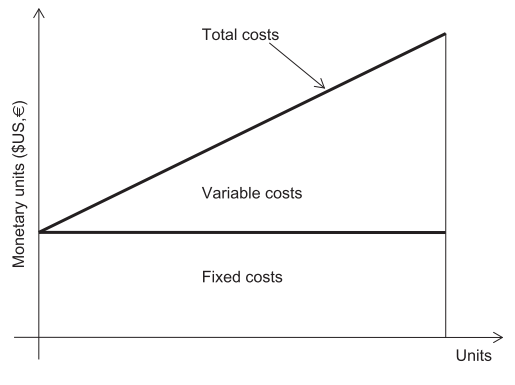
\includegraphics{gfx/fig11.png}\\
The variable costs, that depend on the level of utilization of a given rolling stock/vehicle fleet. They include costs of labor, material, and energy/fuel. These costs are not inevitable. They are lower with the lower utilization of a given rolling stock/vehicle fleet.\\
\par
The total costs $TC(k)$ of any transport company represent the sum of fixed and variable costs, i.e.
\begin{equation}
	\label{total cost}
	TC(k) = FC(k) + VC(k)
\end{equation}
%
Where,\\
\hspace*{10mm}$k$ is the period of time (day, month, quarter, year)\\
\hspace*{10mm}$FC(k)$ is the fixed costs incurred during the time period $k$\\
\hspace*{10mm}$FC(k)$ is the variable costs incurred during the time period $k$\\\\
In addition, the fixed cost of the infrastructure providers and transport operators for construction of infrastructure and acquiring the rolling stock/vehicle fleet are covered by the investments. These, after uniformly spread over the given period of time, usually over the predicted life-cycle, are expected to bring benefits to the actors/stakeholders involved such as investors, transport infrastructure providers and transport operators, users/passengers and freight/goods shippers and receivers, and the local, regional, national, and global community, ie, the economy and society.
%
\subsection{Economies of Scale and Economies of Scope}
The average costs per unit of output are obtained by dividing the total costs (Eq. \ref{total cost}) by the volume of output. The output could be the number of vehicles, the number of passengers, quantity of freight/ goods, the number of vehicle-kilometers, the number of passenger-kilometers, the number of freight-kilometers, etc. If this average cost decreases with increasing of the volume of given output, he economies of scale exist. Otherwise, economies of scope exist. In the former case, in general, the average cost decreases because of spreading the fixed costs over the larger number of units of output. Economies of scale could be interpreted as the cost advantages that companies achieve as a result of size, output, or scale of operations. For example, when the output increases from O1 to O2, the average cost of each unit decreases from AC1 to AC2 as shown in the figure below.\\
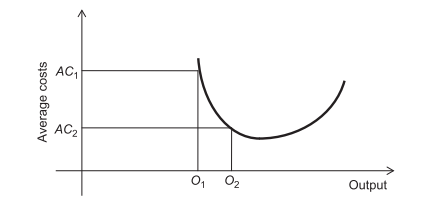
\includegraphics{gfx/fig12.png}\\
Trucking, delivery companies, and airlines usually organize a hub-and-spoke networks as the flows between hubs are characterized by economies of scale. At hubs, goods or passengers are exchanged across vans, trucks, and planes.\\
\par
Based on Eq. \ref{total cost}, the average cost per unit of output can be estimated in the following way:
\begin{equation}
	AC(k) = TC(k)/VO(k) = [FC(k) + VC(k)]/VO(k)
\end{equation}
Where $VO(k)$ is the volume of output during the time period (k) (number, quantity).\\
\par
Transportation projects and transportation operations are also characterized by marginal costs. Marginal costs are defined as the change in total cost caused by supplying an additional unit of transport capacity—transport service, seat at transport service, etc. Marginal costs have a tendency to decrease with transportation project size.\\
\par
Economies of scope are defined as decreasing of the average total cost with increasing of the number of different services produced. In the case of a transport company, this could be offering transport services for both passengers and freight/goods. An airline operating both passenger and cargo aircraft fleet could be an example. Such airline can operate at lower cost than what it would be cost of two separate airlines (one operating passenger aircraft fleet, and the other operating cargo aircraft fleet).
